\section{Related Work}
\label{sec:slam-related-work}
The development of Simultaneous Localisation and Mapping (SLAM) has shifted from laboratory settings to complex, real-world deployments across autonomous driving, aerial vehicles, and subterranean exploration. Due to the limitations of external positioning systems such as GNSS in dynamic or urban environments, Light Detection and Ranging (LiDAR) has become the dominant sensing modality, providing high-fidelity, active 3D geometry independent of ambient illumination. The state of the art in this field is defined by LiDAR-Inertial Odometry (LIO), which tightly couples LiDAR measurements with high-frequency inertial data from an Inertial Measurement Unit (IMU) to compensate for motion distortion and maintain observability in geometrically degenerate scenes \cite{koideGLIM3DRangeInertial2024}. Modern LIO research is primarily distinguished by a bifurcation of techniques into two dominant optimisation philosophies: Error-State Kalman Filtering (ESKF) and Factor Graph Optimisation (FGO). This review traces the architectural evolution of LIO, comparing and contrasting leading algorithms such as LIO-SAM, FAST-LIO2, GLIM, and Super-LIO to synthesise the current trends in computational efficiency and global consistency.

\subsection{Modern LiDAR-SLAM Architectures}
\label{subsec:lidar-slam-architectures}
The foundation of modern LiDAR SLAM rests on the seminal LOAM (LiDAR Odometry and Mapping) framework \cite{zhangLOAMLidarOdometry2014}, which introduced the critical concept of extracting and registering geometric features, specifically classifying points into ``edge'' and ``planar'' surfaces based on curvature. LOAM's split-process architecture separated high-frequency odometry from low-frequency mapping. Subsequent work, such as LeGO-LOAM \cite{shanLeGOLOAMLightweightGroundOptimized2018}, refined this by optimising ground points separately. However, these systems were loosely-coupled and feature-dependent, leading to inevitable drift over long trajectories and fragility in unstructured environments (e.g., foliage or feature-poor corridors).

The transition to tight-coupling was facilitated by the advancement of IMU Pre-integration theory \cite{forsterOnManifoldPreintegrationRealTime2017}. This re-parameterisation allows IMU integration to be expressed as a relative motion constraint (e.g., $\Delta \mathbf{R}_{ij}$) that is independent of the initial velocity and pose estimate, as illustrated in \cref{fig:imuPreintegration}. This innovation decouples the high IMU rate from the optimisation rate, making it computationally feasible for graph-based methods to efficiently optimise state biases and velocities over large time windows.

\begin{figure}[htbp]
    \centering
    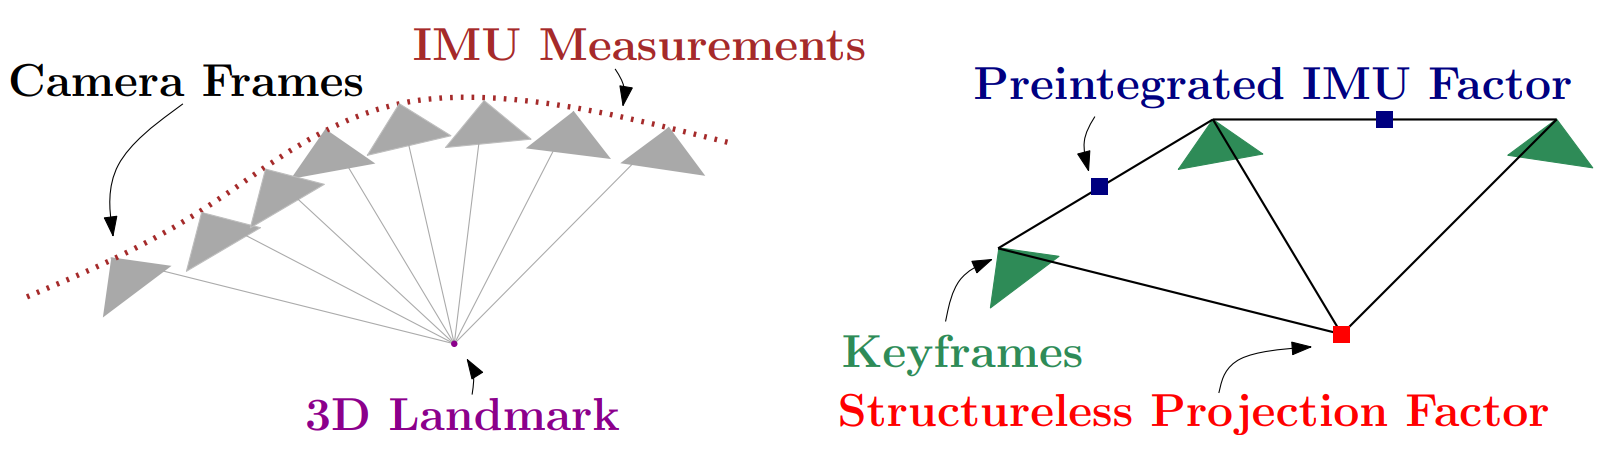
\includegraphics[width=\linewidth]{3-SLAM/3-related-work/figures/imuPreintegration.png}
    \caption{Illustration of on-manifold IMU pre-integration within a sensor-fusion odometry pipeline. Left: raw camera frames and high-frequency inertial measurements arriving asynchronously between keyframes. Right: the equivalent factor graph, in which the batch of intermediate IMU readings between two keyframes is compressed into a single pre-integrated IMU factor, while a structureless vision factor jointly constrains keyframes sharing observations of the same landmark \protect\cite{forsterOnManifoldPreintegrationRealTime2017}.}
    \label{fig:imuPreintegration}
\end{figure}

The result of this evolution is LIO-SAM \cite{shanLIOSAMTightlycoupledLidar2020}, which established the feature-based factor graph benchmark for global consistency, as shown in \cref{fig:liosamArchitecture}. LIO-SAM builds a factor graph incorporating LiDAR odometry, IMU pre-integration, and explicit loop closure factors. To manage computational complexity, it employs a ``sliding window'' local map for scan-to-map matching. Despite its accuracy and robustness compared with its predecessors, its reliance on LOAM-style feature extraction and a standard KD-tree for neighbour searching limits its performance in geometrically degenerate environments.

\begin{figure}[htbp]
    \centering
    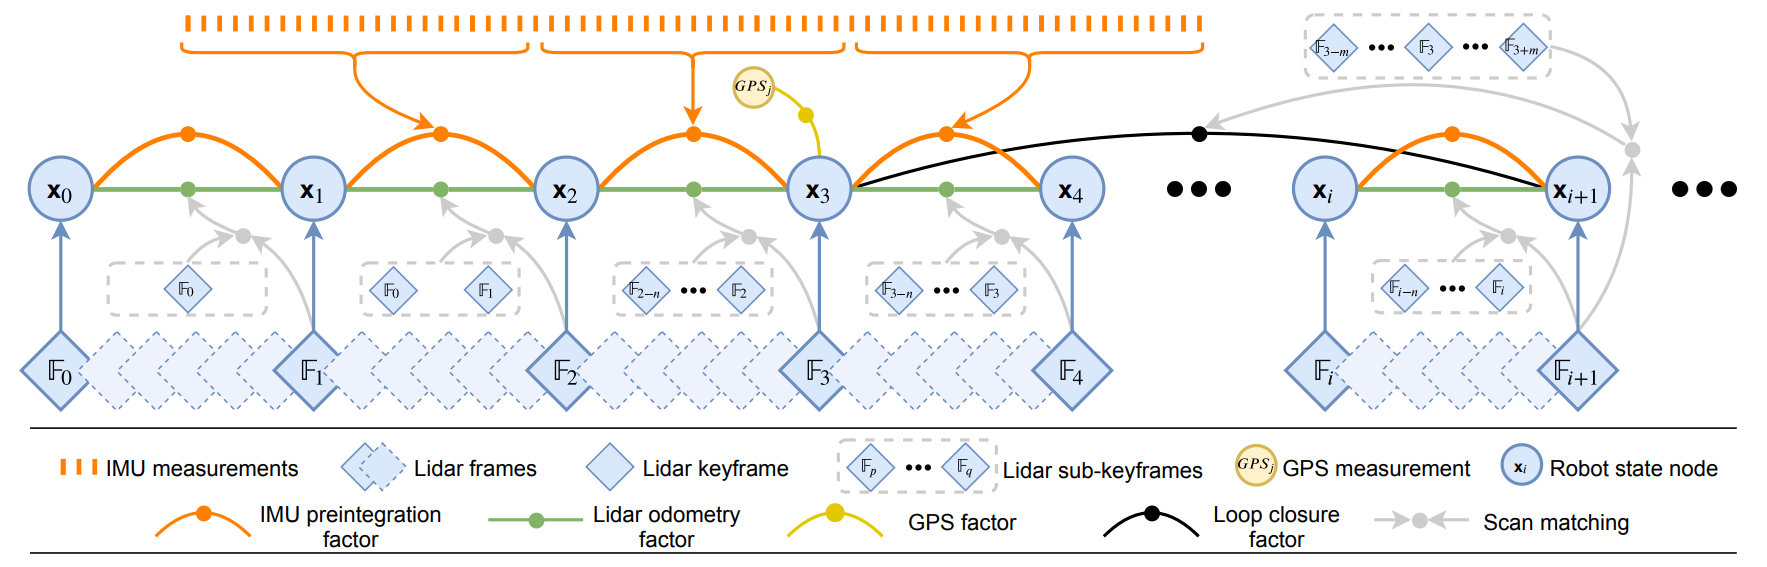
\includegraphics[width=0.85\linewidth]{3-SLAM/3-related-work/figures/LIO_SAM_Archictecture.png}
    \caption{Architecture of the LIO-SAM tightly-coupled LiDAR-inertial odometry framework. Inputs from a 3D LiDAR, an IMU, and an optional GPS receiver are fused within a factor graph composed of four distinct constraint types: IMU pre-integration factors linking consecutive keyframes, LiDAR odometry factors derived from scan-to-local-map registration, GPS absolute-position factors, and loop closure factors that suppress long-term drift \protect\cite{shanLIOSAMTightlycoupledLidar2020}.}
    \label{fig:liosamArchitecture}
\end{figure}

At the time of writing, the state of the art is defined by two architectural tracks: those prioritising extreme computational efficiency via filtering, and those prioritising global consistency and robustness via dense graph optimisation.

\paragraph{Filter-Based Direct Odometry}
Algorithms in the embedded track are designed to minimise CPU usage, making them suitable for low-power ARM processors on platforms like small drones. These systems rely on the Error-State Kalman Filter (ESKF) and are primarily odometry engines that estimate state and covariance, but are susceptible to drift over time as past states are marginalised.

FAST-LIO2 \cite{xuFASTLIO2FastDirect2022} is a widely adopted benchmark for computational efficiency, eschewing feature extraction in favour of registering raw points directly. Its two principal innovations are the Incremental KD-Tree (iKD-Tree), which supports dynamic map updates with amortised $O(\log N)$ complexity, and a Kalman Gain Inversion that reduces the filter update cost from the measurement dimension to the 18-dimensional state vector, enabling kHz-rate processing on modest hardware. Point-LIO \cite{hePointLIORobustHighBandwidth2023} extends this design by updating the EKF state for every individual point as it arrives from the sensor, yielding a processing bandwidth bounded only by the sensor's sampling rate. This point-wise update strategy enables tracking under aggressive motion where conventional scan-accumulation methods fail due to intra-frame distortion. Super-LIO \cite{wangSuperLIORobustEfficient2025} represents the most recent advance in this track, targeting the map data structure rather than the estimator itself. It introduces the \textbf{OctVox} representation — a hybrid combining a spatial hash map with internal octrees — to enforce strict point density constraints, and pairs this with a Heuristic-Guided $k$-Nearest Neighbour (HKNN) search that further reduces per-scan processing time. Reported benchmarks indicate lower CPU utilisation than FAST-LIO2, suggesting OctVox-based representations may define the next generation of resource-constrained LIO.

\paragraph{Graph-Based Global Consistency}
Systems in this track prioritise long-term mapping quality and robustness by leveraging high-performance hardware, particularly embedded GPUs.

GLIM (Global LiDAR Inertial Mapping) \cite{koideGLIM3DRangeInertial2024} represents a distinct departure from CPU-centric design, instead leveraging GPU parallelism to achieve dense, globally consistent mapping, as shown in \cref{fig:glimFramework}. Scan matching in GLIM is implemented via GPU-accelerated Voxelised Generalised Iterative Closest Point (VGICP) factors, which allow the system to incorporate nearly all points per frame and thereby retain geometric constraints that feature-based methods routinely discard. A further key contribution is the Submap Endpoint Mechanism, in which IMU pre-integration factors are inserted as stiff constraints on unobservable degrees of freedom within each submap. This structural guarantee preserves registration quality even when the LiDAR geometry is degenerate — for example in featureless tunnels or elevator shafts. For back-end estimation, GLIM employs a fixed-lag smoother that continuously optimises a bounded window of recent poses, combining the accuracy benefits of iterative re-linearisation with bounded memory consumption, in contrast to full-history SLAM approaches.

\begin{figure}
    \centering
    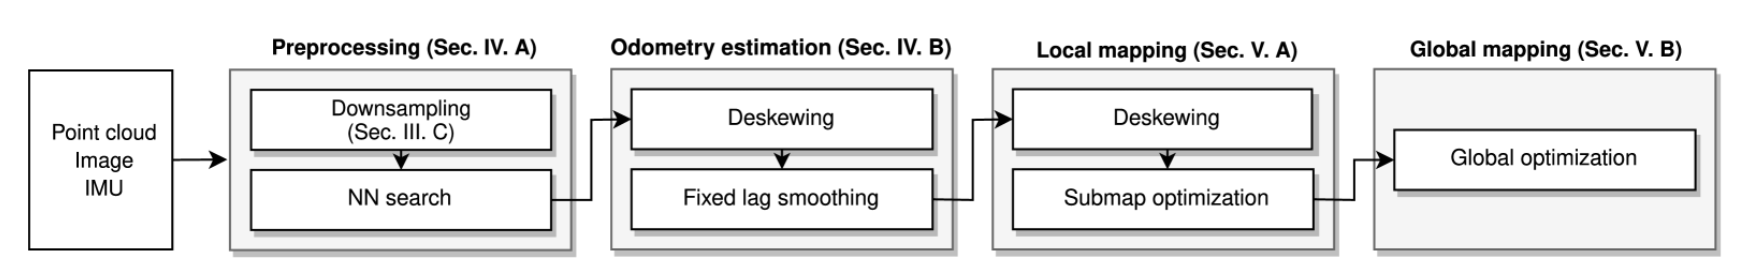
\includegraphics[width=0.9\linewidth]{3-SLAM/3-related-work/figures/glimFramework.png}
    \caption{Overview of the GLIM framework, comprising a preprocessing module and three tightly coupled range-IMU estimation modules. The odometry estimation module deskews point clouds and estimates sensor motion via fixed-lag smoothing; the local mapping module concatenates frames into submaps; and the global mapping module optimises submap poses for long-term global consistency. Each module runs in a dedicated thread \protect\cite{koideGLIM3DRangeInertial2024}.}
    \label{fig:glimFramework}
\end{figure}

This trade-off between computational efficiency and global consistency is summarised in the comparison table below. The most significant recent innovations have occurred in the map data structure domain (iKD-Tree, OctVox) for the filter-based track, and in hardware-software co-design (GLIM's GPU acceleration) for the graph-based track.

\begin{table}[htbp]
\centering
\caption{Comparative Analysis of State-of-the-Art LIO Systems}
\label{tab:comparison}
\small 
\renewcommand{\arraystretch}{1.3} 
\begin{tabular}{@{} l l l c l l @{}}
\toprule
\textbf{Algorithm} & \textbf{Backend} & \textbf{Map Structure} & \begin{tabular}[c]{@{}c@{}}\textbf{Loop}\\\textbf{Closure}\end{tabular} & \begin{tabular}[c]{@{}l@{}}\textbf{Robustness}\\\textbf{(Degeneracy)}\end{tabular} & \begin{tabular}[c]{@{}l@{}}\textbf{Efficiency}\\\textbf{(CPU)}\end{tabular} \\
\midrule
LIO-SAM    & Factor Graph   & Static KD-Tree & Yes & Moderate       & Low             \\
FAST-LIO2  & Iterated ESKF  & iKD-Tree       & No  & High (Direct)  & High            \\
Point-LIO  & Iterated ESKF  & iKD-Tree       & No  & Very High      & Moderate        \\
DLIO       & Geometric Obs. & KD-Tree/iVox   & No  & High           & High            \\
GLIM       & Factor Graph   & GPU Voxelmap   & Yes & \textbf{Extreme} & Low (GPU)       \\
Super-LIO  & Iterated ESKF  & \textbf{OctVox} & No  & High           & \textbf{Very High} \\
\bottomrule
\end{tabular}
\end{table}

Super-LIO is effective for projects constrained to low-power CPUs that can tolerate bounded drift, while GLIM excels at high-fidelity mapping applications where long-term global consistency and robustness to severe degeneracy are paramount, provided a GPU accelerator is available.

\subsection{SLAM Hyperparameter Optimisation}
\label{subsec:slam-hyperparameter}
As hyperparameter optimisation constitutes a primary contribution of this work (see \cref{sec:slam-intro}), this subsection surveys the relevant literature in greater depth than the architecture review above.
The optimisation of SLAM systems has evolved from manual tuning into rigorous hyperparameter optimisation (HPO) and statistical space exploration. In challenging real-world deployments such as agricultural settings, stability, robustness and generalisation become critical design objectives \cite{khanReviewSLAMTechniques2025}. Many modern SLAM systems utilise a complex set of interdependent parameters across the full pipeline, from feature extraction to back-end optimisation. Even focused subsystems such as loop-closure detection can depend strongly on multiple interacting parameters~\cite{hanMultiObjectiveOptimizationLoop2020}. The challenge of configuring a high-dimensional space, often referred to as the curse of dimensionality, poses a significant hurdle in tuning these SLAM systems. The first challenge is finding a subset of points from a high-dimensional search space that accurately represents the underlying performance landscape. 

\paragraph{Search Space Sampling}
One such method for sampling high-dimensional search spaces is Latin Hypercube Sampling (LHS). LHS, as formally introduced by Michael McKay in 1979, was used as a variance reduction technique to address the inefficiencies of Monte Carlo simulation (MCS) in high-dimensional domains \cite{chrismanLatinHypercubeSampling2014}. In MCS, sample points are generated independently, which often leads to ``clusters'' and ``voids'' in disparate regions, which can neglect critical narrow regions of optimal performance \cite{deutschLatinHypercubeSampling2012}. LHS addresses this by enforcing a stratification of the marginal distributions of each input variable.

LHS divides the range of each of the $d$ variables into $n$ equiprobable intervals. In a standard uniform distribution of $[0, 1]$, these strata are defined as $A_i = \left( \frac{i-1}{n}, \frac{i}{n} \right]$ for $i = 1, \dots, n$ \cite{chrismanLatinHypercubeSampling2014}. To generate a LHS sample, one value is drawn from each interval for each dimension. These values are then combined into vectors such that
each $n$ sample point is the only representative in each axis-aligned hyperplane. A visual comparison of MCS and LHS point distributions is shown in \cref{fig:samplingComparison}, and a comparison of LHS, MCS and Grid Search is detailed in \cref{tab:sampling_comparison}.

\begin{table}[h]
\centering
\small
\renewcommand{\arraystretch}{1.5}
\begin{tabularx}{\textwidth}{@{} >{\bfseries}l X X X @{}}
\toprule
Sampling Attribute & \textbf{Monte Carlo (MCS)} & \textbf{Grid Search} & \textbf{Latin Hypercube (LHS)} \\ 
\midrule
Variable Coverage & Random; susceptible to clustering & Uniform but sparse for high $d$ & Guaranteed univariate uniformity \cite{chrismanLatinHypercubeSampling2014} \\ 
\addlinespace
Sample Efficiency & Low; requires large $n$ for stability & Very low; $n^d$ scaling & High; independent of $d$ \cite{deutschLatinHypercubeSampling2012} \\ 
\addlinespace
Bias/Variance & Unbiased; high variance & Biased to grid points & Consistent; asymptotically unbiased \cite{packhamLatinHypercubeSampling2008} \\ 
\addlinespace
Search Structure & Unstructured & Rigidly structured & Near-random with low discrepancy \cite{chrismanLatinHypercubeSampling2014} \\ 
\bottomrule
\end{tabularx}
\caption{Comparison of Sampling Strategies}
\label{tab:sampling_comparison}
\end{table}

\begin{figure}[htbp]
    \centering
    \begin{subfigure}[b]{0.48\linewidth}
        \centering
        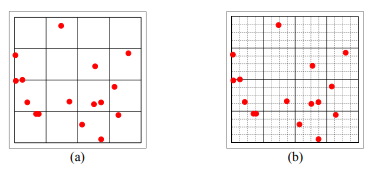
\includegraphics[width=\linewidth]{3-SLAM/3-related-work/figures/MC_dist.png}
        \caption{Monte Carlo sampling}
        \label{fig:mcDist}
    \end{subfigure}
    \hfill
    \begin{subfigure}[b]{0.48\linewidth}
        \centering
        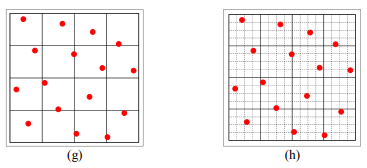
\includegraphics[width=\linewidth]{3-SLAM/3-related-work/figures/LHS_dist.png}
        \caption{Latin Hypercube sampling}
        \label{fig:lhsDist}
    \end{subfigure}
    \caption{Spatial distribution of 16 sample points drawn in a two-dimensional parameter space. In~\subref{fig:mcDist}, pure Monte Carlo sampling populates the space without structural constraint, producing irregular clusters and uncovered voids. In~\subref{fig:lhsDist}, the optimised Latin Hypercube Sampling stratification guarantee ensures that exactly one sample occupies each row and column of the partition grid, yielding substantially more uniform marginal coverage for the same number of evaluations \protect\cite{deutschLatinHypercubeSampling2012}.}
    \label{fig:samplingComparison}
\end{figure}

The advantage of LHS in SLAM parameterisation comes from its capacity to represent the parameter space with fewer samples than traditional methods. In a SLAM system with ten parameters, a grid search with only three levels per parameter would require $3^{10} = 59,049$ evaluations. Testing each sample on a real trajectory quickly becomes time prohibitive. LHS can explore the same search space with fewer points while maintaining that each parameter is tested at different levels \cite{deutschLatinHypercubeSampling2012}. Although uniformity is guaranteed across each axis, this does not guarantee that the interior of the hypercube is filled uniformly. As a result, researchers have developed Latin Hypercube Sampling with Multidimensional Uniformity (LHSMDU) to address the limitations of univariate stratification \cite{deutschLatinHypercubeSampling2012}. LHSMDU employs a sequential elimination process, where a large pool of MCS candidates are generated, and those that are too close in the multidimensional space are pruned \cite{deutschLatinHypercubeSampling2012}. This method maximises the minimum inter-point distance, maximising the spread of samples throughout the multi-dimensional space.

Often the SLAM parameters have physical or co-dependent constraints, such as turn radii or computational resource limits.
Standard LHS assumes independent variables, but extensions like Latin Hypercube Sampling with Dependence (LHSD) allow for the incorporation of copula-based dependence structures \cite{packhamLatinHypercubeSampling2008}. This method enforces constraints on the sampling strategy so that the search does not enter undefined/invalid regions of the search space. 

\paragraph{Robustness, Generalisation and Overfitting}
Finding a high-performance SLAM configuration for a single dataset is straightforward; the challenge is finding one that generalises across diverse environments. Single-dataset optimisation tends to overfit to the specific noise realisations and environmental characteristics of that sequence~\cite{koideAdaptiveHyperparameter2021}. A parameter set tuned for a feature-rich, static environment may adopt aggressive matching thresholds that cause tracking loss or false loop closures in open terrain with sparse landmarks. Environmental factors such as lighting variation, dynamic objects, geometric degeneracy, and platform speed each affect visual and LiDAR SLAM differently, making cross-environment robustness a fundamental constraint on the optimisation strategy. Bayesian optimisation approximates the objective with a probabilistic surrogate and selects evaluation points to maximise expected improvement, providing a sample-efficient, gradient-free framework for this cross-environment hyperparameter search~\cite{kandasamyTuningHyperparametersGrad}. This motivates the multi-dataset consensus framework developed in \cref{subsec:robust-slam-param}, which evaluates candidate configurations across multiple trajectories to penalise over-specialisation.
